\documentclass[titlepage=true]{scrartcl} % bessere form als article

\usepackage{blindtext}

\usepackage{polyglossia} % Sprachen
\setmainlanguage[babelshorthands=true]{german}

\usepackage{enumitem} % Für eigene Symbole in Aufzählungen

% Math
\usepackage{mathtools}
\usepackage{amsmath}


\usepackage{hyperref} % Verlinkt das Inhaltsverzeichnis und erlaubt \url

\usepackage{listings}
\usepackage{color}
\definecolor{mygreen}{rgb}{0,0.6,0}
\definecolor{mygray}{rgb}{0.5,0.5,0.5}
\definecolor{mymauve}{rgb}{0.58,0,0.82}

\lstset{ %
    backgroundcolor=\color{white},   % choose the background color
    basicstyle=\footnotesize,        % size of fonts used for the code
    breaklines=true,                 % automatic line breaking only at whitespace
    captionpos=b,                    % sets the caption-position to bottom
    commentstyle=\color{mygreen},    % comment style
    escapeinside={\%*}{*)},          % if you want to add LaTeX within your code
    keywordstyle=\color{blue},       % keyword style
    stringstyle=\color{mymauve},     % string literal style
}


% \usepackage[outputdir=build]{minted}

% \titlehead{}
% \subject{}
\title{\LaTeX Kurs}
\subtitle{Eine Zusammenfassung}
\author{\textit{Marvin Raiser}}
\date{\today}

\begin{document}

\maketitle

\tableofcontents
\newpage

% Einleitungs Sektion
\section{Einleitung}

\subsection{Geschichte}
1977 entwickelte \textit{Donald E. Knuth} das Textverarbeitungssystem TeX (griechisch texum). \textit{Leslie Lamport} erweiterte TeX mit mehr Abstraktion, starker Vereinfachung und einem spezifischeren Befehlssatz zu LaTeX. Ursprünglich als Darstellungswerkzeug mathematischer Formeln gedacht wurde es schnell auch von zahlreichen Autoren zum einheitlichen Layouten ihrer Werke genutzt.
Darauf aufbauend werden bis heute zahlreiche LaTeX Erweiterungen entwickelt und der Einsatz in Wissenschaft und des Schreibens ist unabdingbar.
\footnote{Aus \url{https://www.selflinux.org/selflinux/html/latex_geschichte01.html}}

\subsection{Wofür ist \LaTeX geeignet?}
Gut geeignet ist \LaTeX aufgrund des einheitlichen hochkonfigurierbaren Layouting,  mathematischen Werkzeuge, Mehrsprachigkeit und Bibliographieerstellung für Schriftstücke mit logischem Aufbau wie z.B. Naturwissenschaftliche Arbeiten, Geisteswissenschaftliche Arbeiten, Artikel, Abschlussarbeiten, sowie Bücher und simple Präsentationen.

\textbf{Nicht} geeignet ist \LaTeX für Dokumente mit wenig Struktur, Präsentationen (bunt, drehend, blinkend, Animationen), Plakate, Dokumente mit vielen uneinheitlichen Bildern.

\subsection{Wie funktioniert \TeX?}

\subsubsection{What You See Is What You Get}
Bei klassischen Texteditoren wie Word schreibt und sieht man genau das was man will und bekommt. Formatierung und Positionierung passiert dabei im Hintergrund automatisch und sieht der User bereits verarbeitet.
Das erleichtert das Schreiben, erschwert jedoch auch das Layouting von großen Dokumenten, da die Eigenschaften intransparent sind.

\subsubsection{What You See Is What You Mean}
Dem \textit{WYSIWYG} steht das \textit{What You See Is What You Mean (WYSIWYM)} entgegen. Dabei wird grundsätzlich zwischen den Textdateien und dem verarbeiteten Ergebnis unterschieden. Die Textdateien sind jedoch mit der zugrunde liegenden Sprache \LaTeX geschrieben (vergleichbar mit einer Programmiersprache). Diese Sprache abstrahiert Layout, Text und sonstige Medien und bringt diese in eine logische Struktur.

\subsubsection{Kompilieren einer \LaTeX Datei}
\begin{figure}[h]
    \centering
    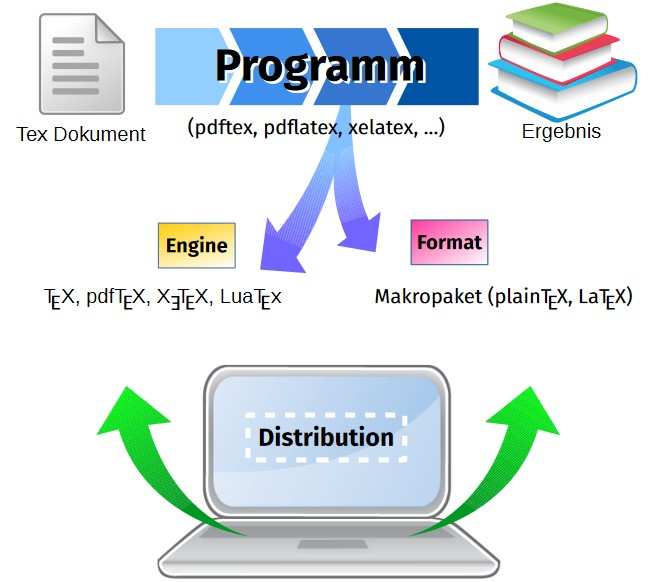
\includegraphics[scale=0.5]{bilder/latex-compiler.jpg}
    \caption{Wie Tex Dokumente kompiliert werden}
    \label{fig.kompiler}
\end{figure}

Diese Sprache und Struktur muss zur gegebenen Zeit verarbeitet und zusammengelegt bzw. \textit{kompiliert} werden, um daraus das gewünschte Resultat, zu generieren. Wie in illustriert sind mehrere Programme zum Kompilieren eines Tex Dokuments notwendig.
Diese Programme setzen sich aus der generellen \TeX Engine und weiteren Makropaketen zusammen die wiederum unterschiedliche Formatierungen reinbringen.
Distributionen sind dabei unterschiedliche Weiterentwicklungen in unterschiedliche Richtungen und Systeme, die aber alle auf der selben Basis aufbauen. In der Regel bringt eine Distribution alle typischen Packete mit die man brauchen wird.
\footnote{Weitere Distributionen und Programme: \url{http://www.tug.org/interest.html}}


\subsection{Das erste Dokument}
Im Folgenden verwenden wir \textit{texlive} als Distribution und \textit{xelatex} als Compiler.
Als Editor ist TextStudiu zu empfehlen. Alternativ kann man auch VS Code mit der Extension \textit{LaTeX Workshop} verwenden.

Beim Erstellen der ersten Datei darauf achten, dass alle Tex Dateien auf \textbf{\textit{.tex}} müssen enden.

\begin{verbatim}
    \documentclass{minimal}
    \begin{document}
    Hallo Welt!
    \end{document}
\end{verbatim}

\newpage

\section{Dokumentheader}
Im \textit{Header} werden einmalig globale Einstellungen getroffen, um unteranderem einheitliches Design zu garantieren oder Packete zu konfigurieren.
Eingeleitet wird der \textit{Header} durch \textit{documentclass} und geschlossen durch \textit{begin(document)}

\subsection{Dokumentklassen}
Dokumentklassen legen erste allgemeine Layoutregeln fest wie beispielsweise Ränder, Abstände, Schriftgrößen etc.
\subsubsection{Typische Klassen}
Die typischen Klassen nach Relevanz und Häufigkeit sortiert. Meist wird \textit{article} verwendet.
\begin{table}[h]
    \centering
    \begin{tabular}{rl}
        article & (Kurze) Artikel          \\
        report  & Reporte, Tagungsberichte \\
        book    & Bücher                   \\
        letter  & Briefe                   \\
        minimal & Minimalbeispiele         \\
        beamer  & Präsentationen
    \end{tabular}
    \caption{Die typischen Dokumentklassen}
    \label{typischeDokumentKlassen}
\end{table}

\subsubsection{KOMA-Klassen}
KOMA-Klassen sind moderne Erweiterungen der typischen Klassen. Sie modernisieren nicht nur das Layout und Design, sondern erlauben es einfach KOMA-Skripte zunutzen, wodurch mehr Funktionalität und Packete unterstützt wird.

\begin{table}[h]
    \centering
    \begin{tabular}{rl}
        scrartcl & Erweiterung von article   \\
        scrreprt & Erweiterung von report    \\
        scrbook  & Erweiterung von book      \\
        scrlttr2 & Sehr mächtige Briefklasse \\
    \end{tabular}
    \caption{Zusätzliche KOMA-Klassen}
    \label{KOMAKlassen}
\end{table}

\subsubsection{Wichtige \texttt{documentclass} Optionen}

\subsection{Titel}

\subsection{Wichtige Pakete}

\newpage

\section{Dokumentstruktur}

\subsection{Abschnitte und Überschriften}

\subsection{Umgebungen}

\subsection{Verzeichnisse}

\subsection{Ausrichtung}

\subsection{Abstände}

\subsection{Zeilen- und Seitenumbrüche}

\newpage

\section{Text}

\subsection{Schriftart}

\subsection{Schriftgröße}

\subsection{Symbole}

\subsection{Trennzeichen und Striche}

\subsection{Datum}

\newpage

\section{Listen}

\subsection{Auflistungen}
\begin{itemize}
    \item Apfel
    \item Birne
\end{itemize}

\subsection{Auflistungen verschachtelt}
\begin{itemize}
    \item Obst
          \begin{itemize}
              \item Apfel
              \item Birne
          \end{itemize}
    \item Gemüse
\end{itemize}


\subsection{Auflistungen mit andere Zeichen}
\begin{itemize}
    \item Apfel
    \item[--] Birne
    \item Erdbeere
\end{itemize}

\subsection{Auflistungen immer mit anderen Zeichen}
\begin{itemize}
    \renewcommand\labelitemi{--}
    \item Apfel
    \item Birne
\end{itemize}

\subsection{Aufzählungen}
\begin{enumerate}
    \item Apfel
    \item Birne
\end{enumerate}

\subsection{Aufzählungen verschachtelt}
\begin{enumerate}
    \item Obst
          \begin{enumerate}
              \item Apfel
              \item Birne
          \end{enumerate}
    \item Gemüse
\end{enumerate}

\subsection{Aufzählungen mit enumitem packet}
\begin{enumerate}[label=(\alph*)]
    \item Apfel
    \item Birne
    \item Banane
\end{enumerate}

\newpage

\section{Abbildungen}
In \LaTeX können auch Bilder eingefügt werden. Hierfür kann \textit{includegraphics} genutzt werden.


\includegraphics[scale=0.8]{bilder/penguin-sleeping.jpg}

Doch oftmals sollen Bilder flüssig und dynamisch dem Text angepasst werden. Mit der Fließumgebungen \textit{figure} kann hierbei einem Bild eine \textit{caption} und ein \textit{label} gegeben werden. Das Label kann im Text referenziert werden.

\begin{figure}
    
\includegraphics[scale=0.3]{bilder/penguin.png}
    \caption{Ein süßer Pinguin in Fließumgebung}
    \label{fig.pinguin}
\end{figure}

Schaut euch den süßen Pinguin in Abbildung \ref{fig.pinguin} an! Doch warum befindet sich dieser so komisch oben? \LaTeX versucht hier die Abbildung an den restlichen Inhalt der Seite anzupassen und plaziert daher das Bild so komisch an den Anfang. Mit der \textit{[h]} Option der \textit{figure} Fließumgebung kann erzwungen werden, dass die Abbildung an der jetzigen Position eingefügt werden soll. Mit \textit{centering} kann der nachfolgende Inhalt, die Abbildung, zentriert werden.

\begin{figure}[h]
    \centering
    
\includegraphics[scale=0.2]{bilder/penguin-family.jpg}
    \caption{Pinguin Familie, awwww}
    \label{fig.pinguinFamily}
\end{figure}

\newpage

\section{Tabellen}

\begin{table}[h]
    \begin{tabular}{ccc}
        a & b & c \\
        A & B & C
    \end{tabular}
    \caption{Das einfache abc}
    \label{tab:abc}
\end{table}

Im Text kann man auf Tabelle \ref{tab:abc} verweisen

\blindtext

\newpage

% Umgebungen und Mathe Sektion
\section{Mathe}

Im \textit{inline} Mathematik-Modus definieren wir die Masse $m$, Energie $E$ sowie die Lichtgeschwindigkeit \(c\), die wir anschließend im \textit{display} Mathematik-Modus einer Formel verwenden

\[
    E=mc^2
\]

Auch Variablen und griechische Symbole sind möglich
\[
    \alpha = \theta \cdot \gamma
\]

Brüche können mit \textit{frac} beschrieben werden
\[
    \alpha = \frac{\beta\cdot\alpha}{\Gamma}
\]

Im Gegensatz zum einfachen \textit{display} Mathematik-Modus sind Gleichungen in der \textit{equation} Umgebung nummeriert.

\begin{equation}
    \int_{0}^{\infty} f(x)\,\mathrm{d}x
\end{equation}

Mit \textit{align} kann man Formeln schön untereinander alignen.

\begin{align}
    a     & = b + c \\
    c + d & = e + f
\end{align}



\subsection{Maxwellgleichung}

In cgs-Einheiten und differentieller Form lauten die vier Maxwellgleichungen:

\begin{align}
    \nabla \cdot \vec{E}  & = 4\pi \rho                                     & \text{Gaußsches Gesetz}                        \\
    \nabla \cdot \vec{B}  & = 0                                             &                                                \\
    \nabla \times \vec{E} & = -\partial_{ct} \vec{B}                        & \text{Faradaysches Induktionsgesetz}           \\
    \nabla \times \vec{B} & = \frac{4\pi}{c}\vec{j} + \partial_{ct} \vec{E} & \text{Ampêre-Maxwellsches Durchflutungsgesetz}
\end{align}




\newpage

\section{Fließumgebungen und Verweise}

\subsection{Fließumgebungen}
Layout, Positionierung, label, caption

\subsection{Referenzieren}
ref, eqref, pageref

\subsection{Abbildungen}
Am Beispiel für eine Abbildung

\subsection{Tabellen}
Am Beispiel für eine Tabelle

\subsection{Mathematik}
Am Beispiel für eine Formel

\subsection{Fußnoten}


\newpage

\section{Sourcecode}

\subsection{lstlisting}

\subsubsection{Java}
\begin{lstlisting}[language=java]
    class HelloWorldApp {
        public static void main(String[] args) {
            System.out.println("Hello World!"); // Display the string.
            for (int i = 0; i < 100; ++i) {
                System.out.println(i);
            }
        }
    }
\end{lstlisting}


\subsubsection{Python} %from http://wiki.scipy.org/Numpy_Example_List
\begin{lstlisting}[language=python]
>>> from numpy import *
>>> from numpy.fft import *
>>> signal = array([-2., 8., -6., 4., 1., 0., 3., 5.])
>>> fourier = fft(signal)
>>> N = len(signal)
>>> timestep = 0.1 # if unit=day -> freq unit=cycles/day
>>> freq = fftfreq(N, d=timestep) # freqs corresponding to 'fourier'
>>> freq
array([ 0. , 1.25, 2.5 , 3.75, -5. , -3.75, -2.5 , -1.25])
>>> fftshift(freq) # freqs in ascending order
array([-5. , -3.75, -2.5 , -1.25, 0. , 1.25, 2.5 , 3.75])
\end{lstlisting}


\subsubsection{HTML}
\begin{lstlisting}[language=html]
    <html>
    <head>
        <title>Hello</title>
    </head>
    <body>Hello</body>
    </html>
\end{lstlisting}

\subsection{minted}

\newpage

\section{Große Projekt Strukturen}

\subsection{Auslagern durch \textit{input} und \textit{include}}

\subsection{Dateistruktur}

\subsection{Versionsverwaltung}

\section{Weiterführende Literatur}



\newpage

\section{Danksagung}
Diese \LaTeX Zusammenfassung ist während dem \LaTeX Kurs des Heidelberger Life-Science Labs am 12. Juni 2021 entstanden.\\
Großes Dankeschön an das Kursleitungsduo Hannes Keppler und Jakob Kreft!

\end{document}